\documentclass[border=1mm]{standalone}

\usepackage{preambletikz}
 
\begin{document}


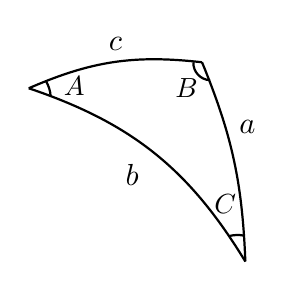
\begin{tikzpicture}[scale=1.1]

\coordinate (A) at (-1,1);
\coordinate (B) at (1,1.3);
\coordinate (C) at (1.5,-1);

\draw[thick, black] (A) to[bend left=15] (B)  node[midway, above, yshift=1.3cm] {$c$};
\draw[thick, black] (B) to[bend left=10] (C)  node[midway, right, xshift=1.3cm, yshift=0.55cm] {$a$};
\draw[thick, black] (A) to[bend left=20] (C)  node[midway, left, xshift=0.4cm] {$b$};
 
\coordinate (BB) at (0.9,1.3);
\draw[thick,black] (BB) arc (178:268:0.2) node[xshift=-3mm, yshift=-1mm, scale=1] {$B$};

\coordinate (AA) at (-0.8,1.08);
\draw[thick,black] (AA) arc (30:4:0.4) node[xshift=3mm, yshift=1.3mm,scale=1 ] {$A$};

\coordinate (CC) at (1.48,-0.7);
\draw[thick,black] (CC) arc (80:104:0.4) node[xshift=-0.5mm, yshift=4mm, scale=1] {$C$};

\end{tikzpicture}


\end{document}










































